\begin{exercises} 
  \item The velocity of an object moving along an axis is given by the piecewise linear function $v$ that is pictured in 
  Figure~\ref{F:4.3.Ez1}.  Assume that the object is moving to the right when its velocity is positive, and moving to the left when its velocity is negative.  Assume that the given velocity function is valid for $t = 0$ to $t = 4$.
\begin{figure}[h]
\begin{center}
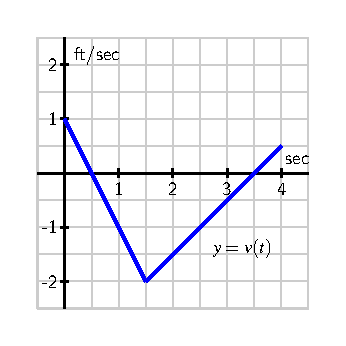
\includegraphics{figures/4_3_Ez1.eps}
\caption{The velocity function of a moving object.} \label{F:4.3.Ez1}
\end{center}
\end{figure} 
	\ba
		\item Write an expression involving definite integrals whose value is the total change in position of the object on the interval $[0,4]$.
		\item Use the provided graph of $v$ to determine the value of the total change in position on $[0,4]$.
		\item Write an expression involving definite integrals whose value is the total distance traveled by the object on $[0,4]$.  What is the exact value of the total distance traveled on $[0,4]$?
		\item What is the object's exact average velocity on $[0,4]$?
		\item Find an algebraic formula for the object's position function on $[0, 1.5]$ that satisfies $s(0) = 0$.
	\ea
	
  \item Suppose that the velocity of a moving object is given by $v(t) = t(t-1)(t-3)$, measured in feet per second, and that this function is valid for $0 \le t \le 4$.
  	\ba
		\item Write an expression involving definite integrals whose value is the total change in position of the object on the interval $[0,4]$.
		\item Use appropriate technology (such as \href{http://gvsu.edu/s/av}{\texttt{http://gvsu.edu/s/a9}}\footnote{Marc Renault, Shippensburg University.}) to compute Riemann sums to estimate the object's total change in position on $[0,4]$.  Work to ensure that your estimate is accurate to two decimal places, and explain how you know this to be the case.
		\item Write an expression involving definite integrals whose value is the total distance traveled by the object on $[0,4]$.
		\item Use appropriate technology to compute Riemann sums to estimate the object's total distance travelled on $[0,4]$.  Work to ensure that your estimate is accurate to two decimal places, and explain how you know this to be the case.
		\item What is the object's average velocity on $[0,4]$, accurate to two decimal places?
	\ea
  
        \item Consider the graphs of two functions $f$ and $g$ that are provided in Figure~\ref{F:4.3.Ez2}.  Each piece of $f$ and $g$ is either part of a straight line or part of a circle.
\begin{figure}[h]
\begin{center}
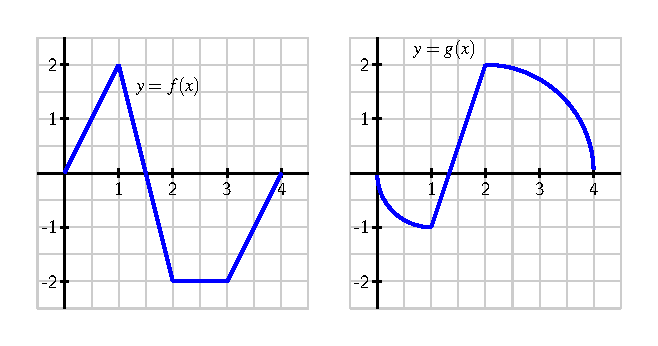
\includegraphics{figures/4_3_Ez2.eps}
\caption{Two functions $f$ and $g$.} \label{F:4.3.Ez2}
\end{center}
\end{figure} 
  \ba
  	\item Determine the exact value of $\int_0^1 [f(x) + g(x)]\,dx$.
	\item Determine the exact value of $\int_1^4 [2f(x) - 3g(x)] \, dx$.
	\item Find the exact average value of $h(x) = g(x) - f(x)$ on $[0,4]$.
	\item For what constant $c$ does the following equation hold?
	$$\int_0^4 c \, dx = \int_0^4 [f(x) + g(x)] \, dx$$
  \ea
  
    \item Let $f(x) = 3 - x^2$ and $g(x) = 2x^2$.
    \ba
    	\item On the interval $[-1,1]$, sketch a labeled graph of $y = f(x)$ and write a definite integral whose value is the exact area bounded by $y = f(x)$ on $[-1,1]$.
	\item On the interval $[-1,1]$, sketch a labeled graph of $y = g(x)$ and write a definite integral whose value is the exact area bounded by $y = g(x)$ on $[-1,1]$.
	\item Write an expression involving a difference of definite integrals whose value is the exact area that lies between $y = f(x)$ and $y = g(x)$ on $[-1,1]$.
	\item Explain why your expression in (c) has the same value as the single integral \\ $\int_{-1}^1 [f(x) - g(x)] \, dx$.
	\item Explain why, in general, if $p(x) \ge q(x)$ for all $x$ in $[a,b]$, the exact area between $y = p(x)$ and $y = q(x)$ is given by
	$$\int_a^b [p(x) - q(x)] \, dx.$$
    \ea
    

\end{exercises}
\afterexercises
